\documentclass[
  degree=bachelor,
  type=design,
  oneside,openany,
  AutoFakeBold=2.5
]{nuaathesis}
% 可用选项:
% degree=[bachelor|master|doctor]   必选,毕业论文学位
% type=[paper|design]   论文类型,本科必选,硕/博默认(强制)论文
% jincheng    可选,将学校信息设置为金城学院
% blankleft   可选,在启用 openright 时,去除空白页的页眉页脚,变成真正的白纸
% msfont      可选,使用微软英文字体
% 其余选项将传给 ctexbook,比较有用的选项有:
% oneside|twoside       可选,单面或双面打印
% openany|openright     可选,在双面打印时,每章的第一页将打印在右侧
% AutoFakeBold          可选,貌似这个数值最接近 M$ Word 的粗体效果
% 推荐:双面打印时,使用 twoside,openright,blankleft;其他场合 oneside,openany

% 写作时,使用这个命令只渲染你想查看的部分,提升工作效率,定稿时注释掉整行
% \includeonly{chapter/00-cover,chapter/30-issues,}

\begin{document}

% 首先,导入论文的基础信息
%# -*- coding: utf-8-unix -*-

% 中文文档信息
\nuaaset{
  title = {基于深度学习的网络流量异常检测算法}, % 论文题目
  author = {闫珺},   % 作者
  studentid = {161420219},  % 学号(本科)
  college = {计算机科学与技术学院},    % 学院,或者(金城)院部
  major = {信息安全},     % 专业(本科)
  classid = {1614204},  % 班号(本科)
  advisors = {皮德常},  % 指导教师
  libraryclassid = {TP371},       % 中图分类号(硕博)
  subjectclassid = {080605},      % 学科分类号(硕博)
  thesisid = {1028704 17-S036},   % 论文编号(硕博)
  majorsubject = {学位论文排版},  % 学科、专业(硕博)
  researchfield = {排版引用},     % 研究方向(硕博)
  % applydate = {二〇一八年五月}  % 默认当前日期
}

% 英文文档信息(本科可以不用写)
\nuaasetEn{
  % college = {NUAA},
  title = {Deep Learning Based Network Traffic Anomaly Detection Algorithm},
  % majorsubject = {Thesis Typesetting},
  % author = {\nuaathesis~Group},
  % advisors = {Prof.~Donald Knuth},
  % applydate = {July, 2017}
}

%% 中文摘要
\begin{abstract}

随着网络的快速发展,网络犯罪所带来的损害越来越大,网络流量异常检测算法主要应用于网络入侵检测系统,是维护网络安全的一种有效的方法。然而网络流量的复杂性与高维度特点,使得开发一种有效的网络流量异常检测算法存在着许多挑战。深度学习的提出克服了这种困难,使得这一问题有了新的解决思路。因此,本文提出了一种基于深度学习的网络流量异常检测算法,首先介绍了深度学习和网络流量异常检测的基础理论,紧接着详细阐述了基于深度学习——DNN模型的关键性技术与思想。接下来,使用KDD Cup 99数据集的训练集和测试集对算法进行了仿真实验与测试,并进行了多组的对比实验选出最适合的模型参数,并对实验结果进行总结分析。结果表明,基于深度学习的网络流量异常检测可以克服网络流量数据的复杂性特点和难以训练的问题,检测准确率相比于浅层机器学习算法有着较大的的提升。

\end{abstract}
\keywords{深度学习, 机器学习, 网络流量异常检测, 网络入侵检测系统}

%% 英文摘要
\begin{abstractEn}
A brief example of paper.
\end{abstractEn}
\keywordsEn{Deep Learning, Machine Learning, Network Traffic Anomaly Detection, NIDS}


\makecover    % 封面
\makedeclare  % 承诺书

\frontmatter  % 启用页眉页脚
\makeabstract % 摘要
\nuaatableofcontents  % 正文目录

\mainmatter   % 以下正文

%# -*- coding: utf-8-unix -*-
\chapter{引言}\label{chap:intro}

\section{研究背景和研究意义}

赛门铁克旗下诺顿公司近日发布的《2017诺顿网络安全调查报告》显示,仅在去年一年,中国网络犯罪受害者的总损失就超过660亿美元,平均每人损失132美元,而每位受害者平均花费近4个工作日(28.3个小时)对攻击所带来的影响进行善后处理。据有关媒体统计,2017年上半年泄露或被盗的数据已经达到了惊人的19亿条。值得一提的是,这一数据已经是2016年泄露数据的总量,全年预计将超过50亿条,其中,仅仅雅虎一家就泄露了多达30亿条。同时,在2017上半年中,全球总共发生了918起网络安全入侵事件,我国用户的信息每年至少被泄露五次。可见,随着互联网的迅速普及,网络安全事件也呈现倍速上升的趋势,它涉及的范围非常广泛,重点主要集中在高校、医疗行业、政府机构以及金融行业等。在互联网在我国急速普及的趋势下,越来越多的人加入了互联网的浩瀚世界,同时也意味承担了这复杂网络世界的风险,网络安全日益成为阻碍中国互联网发展的一股强大的阻力。
网络入侵检测系统(NIDS)是一种有效的维护网络安全的技术,而NIDS的关键性技术就是网络流量异常检测,异常检测指的是在数据中发现不符合正常行为或预期行为的模式的问题。这些不符合预期行为的模式在不同的应用领域通常被称为异常。现今,异常检测的应用非常广泛,例如网络入侵检测系统(NIDS)、信用卡欺诈检测、保险或医疗健康、安全等关键系统的故障检测以及对敌方军事活动的监视等领域。

网络入侵检测系统(NIDS)是网络系统管理员检测组织内部网络各种安全漏洞的重要工具。NIDS监视,分析并发起进入或离开组织网络设备的网络流量的警报,以保证网络系统资源的机密性、完整性和可用性。这种NIDS不同于与被动阻拦外部攻击的防火墙技术,它是一种积极主动的安全防护技术,具有实时性、动态性和主动性等特点,能有效弥补其他静态防御工具的不足。基于入侵检测的方法,NIDS被分为两类:i)基于签名(误 用)的NIDS(SNIDS),以及ii)基于异常检测的NIDS(ADNIDS)。在SNIDS中,例如Snort,其原理是在NIDS中预先安装了定义好的攻击规则,针对安装的规则对流量进行模式匹配以检测网络中的入侵行为,也称为基于先验知识的入侵检测。SNIDS包括基于统计的方法、基于知识的方法和基于机器学习的方法。相比之下,ADNIDS只要观察到偏离了正常流量模式的流量,就会将网络流量归类为入侵,所以也被称之为基于行为的入侵检测系统。SNIDS可以有效检测已知的攻击,其优点是高检测准确度和低误报率。但是,由于规则必须预先安装在IDS中的限制,其表现在检测未知或新类型的攻击时会受到影响。另一方面,ADNIDS非常适合检测未知的、新类型的攻击。虽然ADNIDS容易产生较高的假阳性率,但它在识别新型攻击方面的理论潜力已经引起了研究界的广泛接受。

在为应对未知攻击开发有效和灵活的网络流量异常检测算法方面,主要存在两个挑战。首先,从网络流量数据集中选择用于异常检测的适当特征是困难的。随着攻击场景的不断变化和演变,针对一种类型的攻击所做的检测功能可能并不适用于其他类型的攻击。其次,在真实网络环境下的标签流量数据集很难用于开发NIDS。往往需要付出巨大的努力才能根据一段时间或者实时收集的原始网络流量痕迹生成这样的标签数据集,第二个挑战也正是因为这个原因而形成的。此外,为了保护组织内部网络结构的机密性以及用户的各种隐私信息,网络管理员通常不愿意报告其所管理的网络中可能发生的任何入侵情况。

目前,已经有多种机器学习技术被用于开发ADNIDS,例如人工神经网络(ANN),支持向量机(SVM),朴素贝叶斯 (NB),随机森林(RF),自组织映射(SOM)等等。异常网络流量检测在实现中主要被开发为分类器来区分普通流量和异常流量。许多NIDS会执行特征选择任务,以此从流量数据集中提取相关特征的子集以增强分类结果。特征选择可以去除冗余特征和噪声,有助于降低因冗余特征和噪声导致错误训练的可能性。最近,基于深度学习的方法已经被成功应用于音频、图像和语音处理应用中。这些深度学习方法旨在通过深层网络的复杂抽象来获取到一个良好的数据特征表示,之后,将这些经过复杂抽象的特征应用于监督学习的分类任务中,以此克服浅层机器学习本身存在的问题。可以想象,基于深度学习的方法可以帮助克服开发有效的网络流量异常检测算法的挑战,因此,我选择了深度学习算法来尝试解决网络流量异常检测这一问题。我通过将深度学习模型应用于KDD Cup 99入侵检测数据集来验证基于深度学习的网络流量异常检测算法的可行性。通过多组对比实验寻找用于网络流量异常检测的深度学习模型的合适参数,同时也提供了该深度学习模型与其他技术的比较。

\section{国内外研究现状}
\section{论文的研究内容}
\section{论文的组织结构}
\section{本章小结}
%# -*- coding: utf-8-unix -*-

\chapter{深度学习和网络流量异常检测的基础理论}\label{chap:example}

\section{深度学习}

深度学习技术是机器学习领域研究的最新最火热的成果。自20世纪80年代开始,机器学习技术层出不穷,基于统计模型的感知器、人工神经网络等浅层神经网络,到后来的SVM、最大熵方法等在预测与分类上虽然取得了很好的应用效果,但是,随着互联网的快速发展,数据的数量和维度呈现爆炸式的增长,传统的浅层神经网络面对高维度、复杂数据时表现得力不从心。2006年,多伦多大学的Geoffrey Hinton教授联Ruslan Salakutdinov教授发表了一片开启了深度学习热潮的文章,使得机器学习技术进入了深度学习时代。这篇文章中有两个主要观点:1.多层人工神经网络对于特征学习问题有着非常良好的表现,通过深度学习技术学习到的特征可以对原始数据进行更加本质的刻画;2.深度学习可以克服传统的深层次神经网络在训练时面临的深层误差反馈的消减问题,深度学习可以通过逐层初始化的方法予以克服这一问题,同时,在逐层初始化的过程中,使用的是无监督学习。这使得在大数据时代,数据巨大而标签稀少的情况下,无监督学习的初始化方法有着很好的适用性。深度学习架构(例如DNN、DBN、RNN等)已经被应用至诸多领域,包括语音识别、计算机视觉、自然语言处理、社交网络过滤、音频识别、机器翻译、药物设计和生物信息学等诸多领域。与人类专家相比,在许多情况下它们已经达到了优于人类专家的水平。

\subsection{深度学习的基本思想}

深度学习虽然是计算机领域的技术,但是深度学习与20世纪90年代的由认知神经科学研究者提出的大脑发育理论(尤其是皮层发育理论)是密切相关的。经研究发现,我们人类的大脑的神经元组成了一种较为深层的网络结构,不同层的神经元肩负着不容的任务需要处理。例如,从视觉系统传输过来的信息需要经过多个层次的处理,我们的大脑才能得到正确结果。可以这样想象,在每一层中,我们的大脑的不同层次的神经元可以处理复杂程度不同的信息,浅层的神经元可以处理图像中的局部信息,深层的神经元可以处理图像中更大片区域的信息,信息通过神经元的逐层处理而不断地聚集,同时变得更易于我们大脑分析与处理。深度学习也是如此,如果想要让机器理解更加复杂的问题,模型也需要经过多个层次深度处理才可以。

深度学习是一种机器学习算法:
\begin{itemize}
    \item 适用多层非线性处理单元的级联进行特征提取和转换,每个连续的层使用前一层的输出作为当前层的输入。
    \item 在监督学习(例如:分类)和无监督学习(例如:模式分析)方式下训练。
    \item 学习对应于不同抽象级别的多级表示,这些多级表示构成了深度学习概念的层次结构。
\end{itemize}

深度学习使用了分层的思想,它逐层提取复杂的信号,假设一个具有$n$层的网络结构$A(A_1,A_2,\cdots,A_n)$,它的输入和输出分别是$I$和$O$,表示为:
\begin{equation}
    I \Rightarrow A_1 \Rightarrow A_2 \Rightarrow \cdots \Rightarrow A_n \Rightarrow O    
\end{equation}

如果输出$O$等于输入$I$,那么就可以认为这个模型在经过$n$层变化后是没有损失任何信息的。也就是说,其中的每一层都是原始信息的另一种抽象表示。我们的目的也就是使输入输出尽可能的相似,即输出与输出之间的误差最小。可以发现,这种模式下,深度学习和人的大脑的抽象过程是十分接近的,通过一层一层的抽象,将原始信息组合为机器所能够理解并处理的表示。深度学习的这种抽象是逐层训练的,避免了随着层数增加导致的计算复杂问题。同时,深度学习基于无监督学习的方法可以获取到数据的隐含特征,也并不需要巨量的标记好的数据支持。

深度学习的基本结构如图所示:
\begin{figure}[H]
    \centering
    \includegraphics[width=0.99\textwidth]{structure.pdf}
    \caption{深度学习的基本结构}
    \label{fig:DLstructure}
\end{figure}

\subsection{深度学习的训练过程}

深度学习必然具有比较深的深度,也即比较多的层数,在按传统机器学习方法对深度学习模型进行训练会导致计算异常复杂,计算量变得十分巨大,如果一层一层的训练,又会出现偏差的逐层积累,导致偏差在训练中被不断放大,造成模型的欠拟合。2006年,Geoffrey Hinton教授给出了一种在非监督数据上建立多层神经网络的方法,Hinton教授给出的方法分为如下两个步骤:
\begin{enumerate}
    \item 自底向上的无监督学习

    自底向上的无监督学习,也是深度学习的特征学习过程,第一步,将待训练的训练数据集的特征与标签分离(如果是无标签数据,则不用进行这一步);第二步,深度学习网络对深度学习网络中的第一层使用分离后无标签的训练数据进行训练,使用贪婪无监督的训练方法对其训练,第一层训练完毕后,将第一层训练的结果作为第二层的输入,再次使用上述的无监督学习方法进行训练,依此类推,直至深度学习网络的每一层都训练完毕,此时,我们已经得到了各层的参数了。

    \item 自顶向下的监督学习

    经过自底向上的无监督学习后,深度学习网络使用带标签的训练数据对网络进行进一步训练,由于使用了带有标签的数据对网络进行训练,这一步是监督学习的过程。在自底向上的无监督学习过程中,只能保证各层权值矩阵相对最优而达不到全局最优,所以在自顶向下的监督学习过程中可以将误差从上到下的传递,对每一层的权值矩阵进行微调,从而实现全局最优。那么如何调优呢?Hinton教授使用wake-sleep算法进行调优。先将除去最顶层的其他层之间的权值变为双向的,保证了最顶层是一个单层神经网络,但是其它层转为了图模型。向上的权值表示“认知”,向下的权值表示“生成”。下一步,使用wake-sleep算法调整所有的权值,使得“认知”和“生成”取得一致,这样就确保了生成的最顶层表示可以尽可能的复原底层的节点。例如,如果顶层的一个节点表示这是一个苹果,那么所有的关于苹果的图像就应该激活这个节点,同时这个结点向下生成的图像应该能看起来与苹果类似。
    wake-sleep算法分为wake与sleep两部分:
    \begin{enumerate}
        \item wake:认知过程,借助特征与向上的权值(认知权值)产生每一层的抽象表示,并且,使用梯度下降算法调整每层之间的权值(生成权值)。可以理解为:如果结果与我想象的不一样,改变我的权值使得我想象的结果变为这个样子。
        \item sleep:生成过程,借助顶层表示和向下的权值,生成下层的状态,同时修改每一层间向上的权值。可以理解为:如果通过结果推倒得到的我睡梦中的景象不是我在想象这个结果时产生的景象,那么应该改变我的认知权值使得这种景象在我想象时就是这个样子。
    \end{enumerate}
\end{enumerate}

\subsection{深度学习的优点}

深度学习具有强大的特征学习能力,深度学习的深层结构对复杂数据不仅能起到降维作用,还可以提炼出深层的特征,这意味着我们不需要花费成百上千小时来手工构建、筛选优秀的特征。在这之前,人们花费大量的时间在特征选择这项工作上,甚至有一门专业称为特征选择工程,可见,特征选择的困难是阻碍机器学习发展的一个大问题,而深度学习恰恰可以解决这种问题。另一方面,虽然有监督学习速度较快,效果也很好,但是当今人们每天从社交媒体、硬件和软件服务协议、应用程序许可以及网站cookie中收集到的大量信息都是无标记的,这些信息蕴含了很高的价值可是却没有办法对这些信息进行有效的标注。深度学习网络可以避免这种缺点,因为它在无监督学习中很有优势。

随着硬件方面的巨大进步,也进一步使深度学习成为可能。现代的GPU和TPU每秒可以执行超过万亿次的计算,这使得我们可以在不到一天的时间内训练好一个拥有数百万节点的深度网络。最近,Facebook的研究实验室表示,它们可以在一个小时内学习130万张图片,当然,这恐怖数字的背后需要庞大的计算基础设施支持,但也不难看出目前机器的学习能力是有多么的强大。

深度学习网络可以成功的应用于图像识别、模式识别、基于大数据的知识发现、知识应用和知识预测,而网络流量异常检测这一问题很长一段时间都依赖有专业经验的人手工编写识别规则,使用深度学习让机器自己发现网络流量异常检测规则对于传统方法而言是一个巨大的提升。

\section{网络流量异常检测}

网络异常流量是指网络流量行为偏离其正常行为的情形。随着网络规模不断扩大,复杂性不断增加,网络流量异常对网络的影响也越来越大。准确、快速地检测出网络流量异常,并做出合理的响应,是保证网络安全运行的前提条件之一。

根据对网络异常流量的采集方式,可将网络异常流量检测技术分为:基于网络流量全镜像的检测技术,基于SNMP的检测技术和基于Netflow的监测技术三种常用技术。

基于网络流量全镜像的监测技术,网络流量全镜像采集是目前IDS主要采用的网络流量采集模式,其原理是通过交换机等网络设备的端口镜像或者通过分光器、网络探针等附加设备,实现网络流量的无损复制和镜像采集,和其他两种流量采集方式相比,流量镜像采集的最大特点是能提供丰富的应用信息。

基于SNMP的流量信息采集,实质上是通过提取网络设备Agent提供的MIB(管理对象信息库)中收集一些具体设备及流量信息有关的变量。

基于Netflow的流量检测技术是基于网络设备提供的Netflow机制实现的网络流量信息采集,在此基础上实现的流量信息采集效率和效果均能够满足网络异常流量检测的需求。

而对于异常流量的识别上,同样也有一些理论。虽然IPSec的引入对伪造数据包的DoS和DDoS攻击有较好的防御效果,但是由于其计算量十分巨大,在面对大批伪造报文的攻击时也会造成自身的DoS。目前来说,使用异常检测法是目前的主流和发展方向。其核心在于对流量包的特征分析及其变化,来对流量进行检测。但是就现在而言,大多数还停留在对协议的分析和研究上。

基于SVM的网络流量异常检查系统,在改进的SMO算法基础上进一步提高了检查网络流量异常的时间和精确度。主要研究的是以支持向量机为核心模块构建一个网络流量异常检测系统。

基于活跃熵的网络异常流量检查方法将监控的目标网络是位一个整体系统,对进出的网络数据流所形成的NetFlow记录进行分析,分别统计二者的活跃度并计算他们的活跃熵。

基于流量状态特性的网络异常流量检测模型研究——混合二次网络状态$G(X^2,DKS,DKKS,DAKS)$模型。该模型从动态性原则以及降低误检率和漏检率思想出发,改进原有统计模型,建立了可以动态设定描述网络流量状态参数的加权统计模型。可以更大程度上提高异常检查性能,降低误检率和漏检率。

随着网络的快速发展以及攻击方式的不断革新,当下急需对网络流量异常检测方法,对入侵检测技术进行革新与研究。目前,有如下几种发展方向:
\begin{enumerate}
    \item 高速网络入侵检测:如今网络流量数据呈现爆发式的增长,在带宽越来越高的情况下,数据也随之变得越来越大,尤其是视频数据占用了一大部分带宽,传统的检测方法在速度方面已存在明显不足,因此,研究如何使用高速的流量检测成为了一种发展趋势。
    \item 数据库入侵检测:目前对数据库的入侵行为占比一直居高不下,每年有数十亿条用户数据通过数据库泄露出去,研究如何检测数据库入侵的网络流量是目前情况下非常需要的。
    \item 无线网络入侵检测:随着移动设备尤其是智能手机的飞速发展,无线网络的需求也不断扩大,目前,在很多大城市已经实现了无缝的无线网络覆盖。然而,随着无线网络的快速发展,其自身的安全问题却迟迟止步不前,因此,将异常流量检测技术对于无线网络中的检测,也是一大发展趋势。
    \item 智能化入侵检测:人工智能是目前最火热的技术,在各行各业有着非常成功的应用,已经有很多的机器学习技术应用到了网络流量异常检测中,有神经网络、粒子群算法、人工免疫等等。人工智能技术通过不断地自我学习与更新,可以发现深层次的逻辑表征,实现网络流量异常检测技术的自动匹配与优化。本文也是基于这个发展方向,将深度学习技术应用于网络流量异常检测中,以期取得较传统技术更好的效果,探索深度学习在这个方向的应用的可能性。
\end{enumerate}

\section{本章小结}

本章在第一节对深度学习的基本思想、训练过程以及深度学习的优点进行了详细的阐述,解释了这一技术的基本原理。第二节叙述了网络流量异常检测技术的具体内容、常用方法以及未来的发展趋势。这些内容为下一章介绍技术细节时做了铺垫,有助于更好地理解。

%# -*- coding: utf-8-unix -*-

\chapter{基于深度学习的网络流量异常检测算法改进与实验}

\section{基于深度学习模型——DNN模型的改进}\label{txt:FreqCmd}

\subsection{BP神经网络}

\subsection{Dropout层}

\subsection{Mini-batch}

\subsection{Batch-Normalize}

\subsection{随机梯度下降算法}

\section{算法流程}

\section{实验数据集}

\subsection{数据集介绍}

\subsection{数据预处理}

\section{本章小结}

%# -*- coding: utf-8-unix -*-

\chapter{对比实验和结果分析}

\section{实验数据集的选择}

上一章的最后一节已经介绍了KDD Cup 99数据集,并且说明了对数据的预处理步骤,在最后介绍了本文将使用KDD Cup 99数据集中的“KDD 10\%”和“corrected”这两个数据集作为训练和测试数据集。这一节将详细说明一下这两个数据集在实验中各自的用途。

首先,我选择了完整训练数据集的10\%的数据集作为我的训练数据集,考虑了如下两个原因:一是将完整的训练数据集用于训练使得我的训练时间延长了10倍以上(鉴于使用的个人电脑计算能力有限),二是在基于深度学习的网络流量异常检测算法的实现过程中,我在其他参数相同的情况下对比了使用完整训练数据集以及使用完整训练数据集的10\%作为训练数据集的情况下,模型的准确率相当,经完整训练数据集训练后的模型仅仅比使用10\%数据进行训练后的模型的准确率提高了0.001\%,而训练时间却增加了10倍不止。所以,我选择了数据量较为小的数据集作为训练数据集。

关于测试集的选择,阅读了一些文献发现,有一些文献中的测试集选择的同样是训练数据集,只是将训练数据集分割了,其中70\%-75\%的数据用于训练,25\%-30\%的数据用于测试。这种选择虽然在一些其它数据集上很常见,因为其它数据集只有唯一一个训练数据集,但是对于KDD Cup 99数据集来说,我认为应该将corrected数据集作为测试数据集。首先,corrected数据集本身就是设计者专门收集用于测试的,其次,使用包含未知攻击类型的数据集进行测试可以更好的测试我们所构建的模型的泛化能力。从已知攻击类型学习到检测未知攻击类型的异常流量这一能力正是网络流量异常检测算法研究所迫切需要的。当然,也不能否认训练、测试都在训练数据集中的这种方法所体现的机器学习的强大抽象、学习、分类能力。

因此,在实验中我选择使用KDD 10\%的数据对模型进行训练,corrected测试数据集对模型进行测试。同时,在最后的一组实验中,我也给出了使用从训练数据集分割出来部分数据进行测试的准确率。

\section{实验平台}

本章实验是在macOS High Sierra 10.13.4操作系统上进行的,开发语言使用了Python3,Python版本号是3.6.4。硬件平台CPU型号是Intel Core i5-5257U,双核心四线程,CPU主频是2.7GHz,最大可以睿频到3.1GHz,内存为8GB的DDR3内存,内存频率为1867MHz。

\section{实验过程和结果分析}

在对训练数据集和测试数据集预处理后,得到了$494021 \times 122$和$311029 \times 122$维的输入数据。这两组数据将用于对模型的训练和测试。在训练数据中,将随机抽取其中的25\%出来作为验证集。验证集在训练中不会被训练到,仅仅用于调超参数。

本实验进行了多组控制变量的对比实验,在前一个实验当中表现最好的结构将用于下一组实验中,最终通过多组的对比试验构建出表现较为优秀的模型用于网络异常流量检测。

\subsection{模型深度与节点数目的选择}

在本节实验中,本文进行了多次实验,每次实验构建的深度学习网络结构的层数或节点数都是不相同的,通过多次实验的比对,得到了不同层数对应的准确率汇。除了网络参数不同外,其他参数相同,其他参数分别为:
\begin{itemize}
    \item batchsize: 512
    \item dropout: 0(即不使用dropout)
    \item 激活函数: relu
    \item 优化算法: nadam
    \item 损失函数: categorical\_crossentropy
\end{itemize}

测试结果汇总如下:
% Table generated by Excel2LaTeX from sheet 'Sheet2'
\begin{table}[htbp]
	\centering
	\caption{不同网络参数的实验结果}
	\begin{tabular}{c|c|c|c|c}
		\toprule
		模型序号 & 网络参数             & 准确率  & params  & time      \\
		\midrule
		model1-1   & 24-256-512-256-5     & 92.44\% & 273549  & 22s/epoch \\
		\midrule
		model1-2   & 12-128-256-128-5     & 92.10\% & 69705   & 10s/epoch \\
		\midrule
		model1-3   & 48-512-1024-512-5    & 73.90\% & 1083669 & 72s/epoch \\
		\midrule
		model1-4   & 12-24-48-24-5        & 91.99\% & 4289    & 6s/epoch  \\
		\midrule
		model1-5   & 6-12-24-12-5         & 91.44\% & 1499    & 5s/epoch  \\
		\midrule
		model1-6   & 3-6-12-6-5           & 90.86\% & 590     & 5s/epoch  \\
		\midrule
		model1-7   & 24-512-256-5         & 92.32\% & 148365  & 15s/epoch \\
		\midrule
		model1-8   & 24-256-512-256-128-5 & 92.07\% & 305805  & 24s/epoch \\
		\midrule
		model1-9   & 10-50-10-5           & 91.96\% & 2345    & 5s/epoch  \\
		\bottomrule
	\end{tabular}%
	\label{tab:exp1-1}%
\end{table}%

\begin{figure}[H]
    \centering
    \includegraphics[width=0.99\textwidth]{exp1.pdf}
    \caption{网络参数-准确率结果}
    \label{fig:exp1-2}
\end{figure}

\subsection{batchsize大小的选择}

在上一节的实验中,可以发现,模型model1-1的网络参数取得了最好的测试成绩,同时它的训练时间也比较短,故本节实验在model1-1的网络参数的基础上,测试batchsize大小的选择对模型表现的影响。下面的图表是模型的网络参数为“24-256-512-256-5”的基础上不同batchsize的实验结果:
% Table generated by Excel2LaTeX from sheet 'Sheet2'
\begin{table}[htbp]
	\centering
	\caption{不同batchsize的实验结果}
	\begin{tabular}{c|c|c|c}
		\toprule
		模型序号 & batchsize & 准确率  & time       \\
		\midrule
		model2-1 & 512       & 92.12\% & 23s/epoch  \\
		\midrule
		model2-2 & 256       & 92.16\% & 27s/epoch  \\
		\midrule
		model2-3 & 128       & 92.44\% & 37s/epoch  \\
		\midrule
		model2-4 & 64        & 92.24\% & 57s/epoch  \\
		\midrule
		model2-5 & 32        & 92.51\% & 98s/epoch  \\
		\midrule
		model2-6 & 16        & 92.26\% & 185s/epoch \\
		\midrule
		model2-7 & 8         & 92.43\% & 360s/epoch \\
		\midrule
		model2-8 & 1024      & 92.39\% & 20s/epoch  \\
		\midrule
		model2-9 & 2048      & 92.67\% & 19s/epoch  \\
		\bottomrule
	\end{tabular}%
	\label{tab:exp2-1}%
\end{table}%

\begin{figure}[H]
    \centering
    \includegraphics[width=0.99\textwidth]{exp2.pdf}
    \caption{batchsize-准确率结果}
    \label{fig:exp2-2}
\end{figure}

\subsection{优化算法的选择}

在上一节的实验中,可以发现,模型model2-9的batchsize取得了最好的测试成绩,故本节实验在model2-9的batchsize大小以及model1-1的网络参数的基础上,测试不同的优化算法的选择对模型表现的影响。下面的图表给出了不同优化算法对模型表现的影响:
% Table generated by Excel2LaTeX from sheet 'Sheet2'
\begin{table}[htbp]
	\centering
	\caption{不同优化算法的实验结果}
	\begin{tabular}{c|c|c|c}
		\toprule
		模型序号 & 优化算法 & 准确率  & time      \\
		\midrule
		model3-1 & Nadam    & 92.67\% & 19s/epoch \\
		\midrule
		model3-2 & SGD      & 90.67\% & 18s/epoch \\
		\midrule
		model3-3 & RMSprop  & 92.39\% & 19s/epoch \\
		\midrule
		model3-4 & Adagrad  & 91.91\% & 18s/epoch \\
		\midrule
		model3-5 & Adadelta & 91.71\% & 19s/epoch \\
		\midrule
		model3-6 & Adam     & 92.16\% & 19s/epoch \\
		\midrule
		model3-7 & Adamax   & 91.83\% & 19s/epoch \\
		\bottomrule
	\end{tabular}%
	\label{tab:exp3-1}%
\end{table}%

\begin{figure}[H]
    \centering
    \includegraphics[width=0.99\textwidth]{exp3.pdf}
    \caption{优化算法-准确率结果}
    \label{fig:exp3-2}
\end{figure}


\subsection{不同分类精度下模型的表现}

从第三章对KDD Cup 99数据集的介绍中得知,每一条数据都被标记为正常(Normal)或者异常(Attack),异常类型的数据被细分为4大类共39种攻击类型,其中22种攻击类型出现在了训练数据集中,其它的17种未知攻击类型被收纳在测试数据集中。由于有17种类型的攻击数据只在测试集中出现,而在整个模型的实现以及测试过程中,需要对标记数据提前进行编码,所以即使将39种攻击类型都提前编码,在测试时模型也无法输出超出其本身23种(1种正常标记和22种攻击类型标记)编码范围的结果。所以,本实验将数据的标记进行了整理,分为了两种类型:
\begin{enumerate}
    \item 五分类:NORMAL,PROBE,DOS,U2R,R2L这五类标记代表了所有的39种攻击以及正常流量。模型将对输入的数据给出五种之中的一种。
    \item 二分类:Normal,Attack分别用0,1表示。模型只在(0,1)这两个数字中给出结果。也是网络流量异常检测最基本的功能,即区分正常流量和异常流量。
\end{enumerate}

那么,对于五分类以及二分类这两种不同的分类情况,模型的准确率会有很大的差别吗?下面的实验结果给出了答案。在实验中,按原有的网络结构对二分类进行训练得到了准确率仅为80.52\%的结果。在实验中本文尝试了使用不同的模型参数都无法将准确率提升到前几个实验的90\%以上的准确率级别。从第三章我们了解到使用Dropout技术可以克服深度神经网络的训练困难,因此,这里将Dropout技术应用到了模型中,具体的做法是在除输出层外的每一层之后添加Dropout层,Dropout的值设置为了0.5。使用了Dropout技术后继续进行实验,二分类的准确率达到了五分类的同一水准。具体实验数据请看下面的图表:
% Table generated by Excel2LaTeX from sheet 'Sheet2'
\begin{table}[htbp]
	\centering
	\caption{二分类与五分类的实验结果}
	\begin{tabular}{c|c|c|c}
		\toprule
		分类情况 & 准确率  & dropout & 网络参数         \\
		\midrule
		二分类1  & 80.52\% & 0       & 24-256-512-256-1 \\
		\midrule
		二分类2  & 92.04\% & 0.5     & 24-256-512-256-1 \\
		\midrule
		五分类1  & 92.67\% & 0       & 24-256-512-256-5 \\
		\midrule
		五分类2  & 91.66\% & 0.5     & 24-256-512-256-5 \\
		\bottomrule
	\end{tabular}%
	\label{tab:exp4-1}%
\end{table}%

\begin{figure}[H]
    \centering
    \includegraphics[width=0.99\textwidth]{exp4.pdf}
    \caption{不同分类级别-准确率结果}
    \label{fig:exp4-2}
\end{figure}

\subsection{训练与测试同在KDD 10\%数据集的情况}

当使用KDD 10\%数据集的75\%的数据用于训练本文的深度学习模型,使用KDD 10\%数据集的剩余25\%的数据用于测试时,本文的深度学习取得了相当高的准确率,准确率达到了惊人的99.92\%。下面两图为过程中的具体情况:
\begin{figure}[H]
	\centering
	\begin{subfigure}{.45\textwidth}
		\centering
		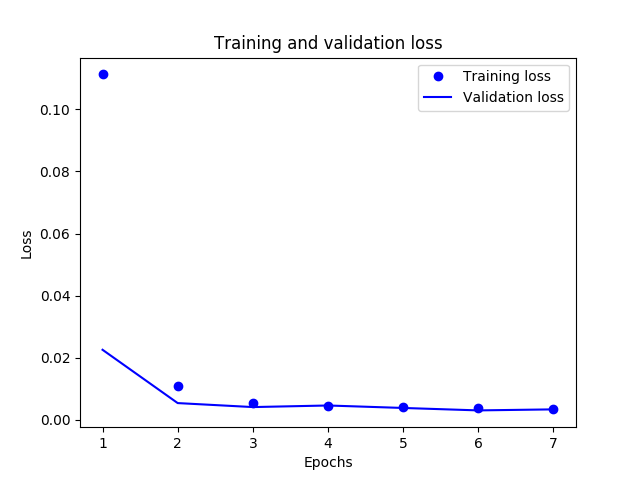
\includegraphics[width=.9\linewidth]{loss-train.png}
		\caption{训练与验证loss变化}
		\label{fig:loss}
	\end{subfigure}
	\begin{subfigure}{.45\textwidth}
		\centering
		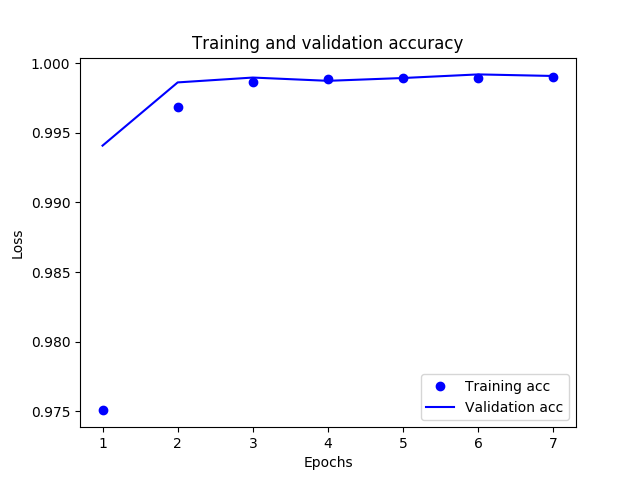
\includegraphics[width=.9\linewidth]{accuracy-train.png}
		\caption{训练与验证accuracy变化}
		\label{fig:acc}
	\end{subfigure}
	\caption{75\%训练-25\%测试的结果}
	\label{fig:test_subfigure}
\end{figure}


这么高的准确率展现了深度学习强大的学习能力。在训练数据集和测试数据集与本实验相同的情况下,陈万志,李东哲等人在文献\cite{r10}中使用了一种将白名单和PSO-BP神经网络过滤有机融合的方法,准确率为87.31\%。文献《基于深度置信网络的入侵检测研究-安琪》中使用了深度置信网络(DBN)达到的准确率为95.55\%\cite{r9}。
  
\subsection{结果分析}

从上面给出的多组对比试验的结果来分析,model1-1的网络参数“24-256-512-256-5”所达到的准确率最高,同时其训练时间也在可接受范围之内。继续增加每层的节点数,准确率下降到了73\%,可见并不是网络节点数越多效果越好。相反,将网络节点数降低一些,却不会发生向增加网络节点数那种情况的准确率大幅度下降,从图表中可知,不同节点数、不同网络层数的情况下,深度学习模型的准确率在90\%-92\%之间浮动。同时可依发现,深度学习模型的参数数量明显影响着深度学习网络的训练速度。

对于batchsize的选择,从实验结果可以发现,在网络结构调整为较为优秀的情况下,batchsize的大小主要影响的是深度学习网络的训练速度。从实验结果的数据中可以发现,batchsize越大,训练速度也就越快。当然batchsize也不能无限的增大,在实验测试时,当我将batchsize设置的非常大时(针对这个数据集,设置了16384),训练速度反而降低了,几乎与batchsize为256时的速度一样,同时,模型的收敛速度也变慢了。这一结果与第三章对mini-batch的分析一致。因此,在应用时,应当根据数据集的规模等因素尝试不同大小的batchsize,直至选择出准确率与训练时间都较好的大小。

对于优化算法的选择,不同模型适合不同的优化算法,在本实验所构建的深度学习模型上,Nadam优化算法的表现最好。同时,RMSprop优化算法也有着不错的表现。在上述实验中,除了优化算法对比试验使用了不同的优化算法,在其它实验中的优化算法都使用了Nadam,下面给出Nadam在本实验中所使用的详细参数供参考。
\begin{itemize}
	\item 学习率lr: 0.002。
	\item beta\_1/beta\_2: 0.9/0.999,通常选取接近于1的数值。
	\item 模糊因子epsilon: None,不使用。
	\item schedule\_decay: 0.004
\end{itemize}

对于二分类与五分类的情况,在不使用Dropout技术时,五分类的准确率较高,达到了92\%以上,然而,二分类的表现很糟糕,只有80\%左右,可见并没有训练好。在加入了Dropout技术并取Dropout值为0.5后,二分类的准确率提高到了92\%以上,和五分类为同一水准。可见,Dropout技术在深度学习的训练上的效果是十分突出的。

在最后,本文也给出了只使用训练数据集进行训练和测试的准确率,这种情况下,测试集不包括未知类型的攻击,都是已知类型的攻击,从结果来看,本文的深度学习模型在这种情况下拟合的非常好,曲线符合一个训练优秀的模型应当展现的曲线。测试的准确率也比文献中的另外两种方法高。

对于训练集和测试集分别使用KDD 10\%训练集和corrected测试集的情况(也是本文大部分实验所使用的情况),在测试集上的准确率最高为92.67\%。可见本文提出的基于深度学习的网络流量异常检测算法模型的检测能力是非常不错的,并且具有不错的泛化能力。

\section{本章小结}

本章是对前面所叙述的基于深度学习的网络流量异常检测算法的实验及实现。首先详细说明了实验数据集各用于训练或是测试环节中,并同时给出了详细的解释。然后给出了实验平台的详细信息,供对比和参考。紧接着分多个部分给出了多组对比试验及其结果,并在最后一部分中对实验结果进行了详细的分析,总结得出的结论。通过本章内容,揭示了本文所提出的算法的应用可能性。
\chapter{总结与展望}

\section{总结}

\section{展望}

\backmatter   % 正文后无编号部分,
\bibliographystyle{nuaathesis}   % 参考文献的样式
\bibliography{bib/sample}   % 参考文献

%# -*- coding: utf-8-unix -*-

\chapter[致谢]{致\hskip\ccwd{}谢}

四年的大学生活随着学位论文的完成进入收尾阶段,此时此刻我感慨良多。学位论文的完成,不仅是自己不断努力进取的成果,更与学院的悉心栽培,老师的细心指导,同学的互助支持分不开。在此之际,我首先要衷心地感谢我的毕业设计导师皮德常老师,在毕业设计期间,皮老师定期安排很长的时间找我面谈,询问毕业设计的进度以及遇到的困难,并给出下一步的研究方向。皮老师的专业知识非常丰富,他的专业指导帮助我解决了很多研究中遇到的问题。我不仅在皮德常老师这里学到了专业的研究知识,还有高效的工作方法和严谨的治学态度,为我以后的学习和工作打下了良好的基础。

感谢和我同一个导师组的李彬和李菠同学,在毕业设计期间,与你们的交流讨论带给我很多灵感和启发。感谢在四年的学习生活中指导和帮助过我的的全体老师和同学。

\end{document}
